\documentclass[border = 3mmm]{standalone}
\usepackage{pgfplots}
\pgfplotsset{width=10cm,height=3.4cm,compat=newest}
\begin{document}
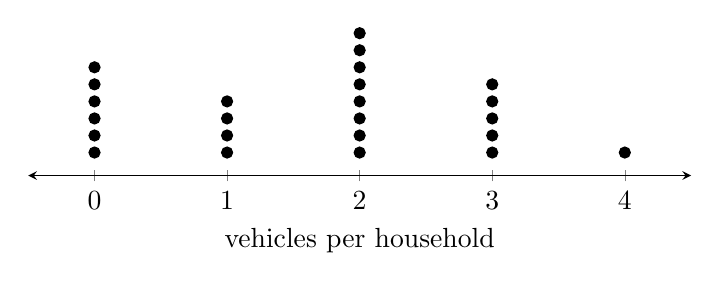
\begin{tikzpicture}
\begin{axis}[
xmin=-0.5,
xmax=4.5,
% hide y axis,
axis y line=none,
axis x line=bottom,
axis x line shift={4pt},
every outer x axis line/.append style={stealth-stealth},
title={},
xlabel={vehicles per household}]
\addplot [only marks, black, mark=*, mark size=2pt] coordinates{(0, 1)(0, 2)(0, 3)(0, 4)(0, 5)(0, 6)(1, 1)(1, 2)(1, 3)(1, 4)(2, 1)(2, 2)(2, 3)(2, 4)(2, 5)(2, 6)(2, 7)(2, 8)(3, 1)(3, 2)(3, 3)(3, 4)(3, 5)(4, 1)};
\end{axis}
\end{tikzpicture}
\end{document}